\documentclass[a4paper,12pt]{article}
\usepackage{graphicx}
\usepackage{xcolor}
\usepackage{tcolorbox}
\usepackage{geometry}
\usepackage{amsmath}
\usepackage{caption}
\usepackage{datetime}

\geometry{margin=1in}

\begin{document}

% ---------- COVER PAGE ----------
\begin{titlepage}
    \centering

    
\includegraphics[width=0.25\textwidth]{IMAGEs/Parlar-logo.png}\par\vspace{1.5cm}
    
    \vspace*{3cm}
    
    {\Huge\bfseries Operational Amplifier Testing Manual \par}
    \vspace{0.5cm}
    {\Large\itshape For LM324 and LM358\par}
    
    \vspace{1.5cm}
    
    {\Large\textbf{Instruction Manual for Test Device and Quality Control}\par}
    
    \vspace{2cm}
    
    \begin{flushleft}
    \textbf{Prepared by:} Alireza Rajabi\\
    \textbf{Approved by:} Mr. Moallemi / Mr. Asadghi\\
    \textbf{Organization:} Parlar Electronics – R\&D Department\\
    \textbf{Document Revision:} 07\\
    \textbf{Date:} \today
    \end{flushleft}
    
    \vfill
    
    \begin{center}
        \textit{This document is prepared in accordance with ISO 9001:2015 and IATF 16949 standards.}
    \end{center}
\end{titlepage}

% ---------- IMPORTANT NOTICE ----------
\begin{tcolorbox}[colback=red!5!white, colframe=red!75!black, title=Important Notice]
This manual contains standardized test procedures for verifying key performance parameters of operational amplifiers (LM324, LM358). 
It is essential to follow all instructions accurately to ensure valid test results. Only qualified personnel should operate the device. 
Data accuracy and integrity must be maintained throughout the testing process.
\end{tcolorbox}

\vspace{1em}

\section{Input Offset Voltage Measurement (V\textsubscript{OS})}

To measure the input offset voltage of an op-amp, the following circuit is used:

\begin{center}
  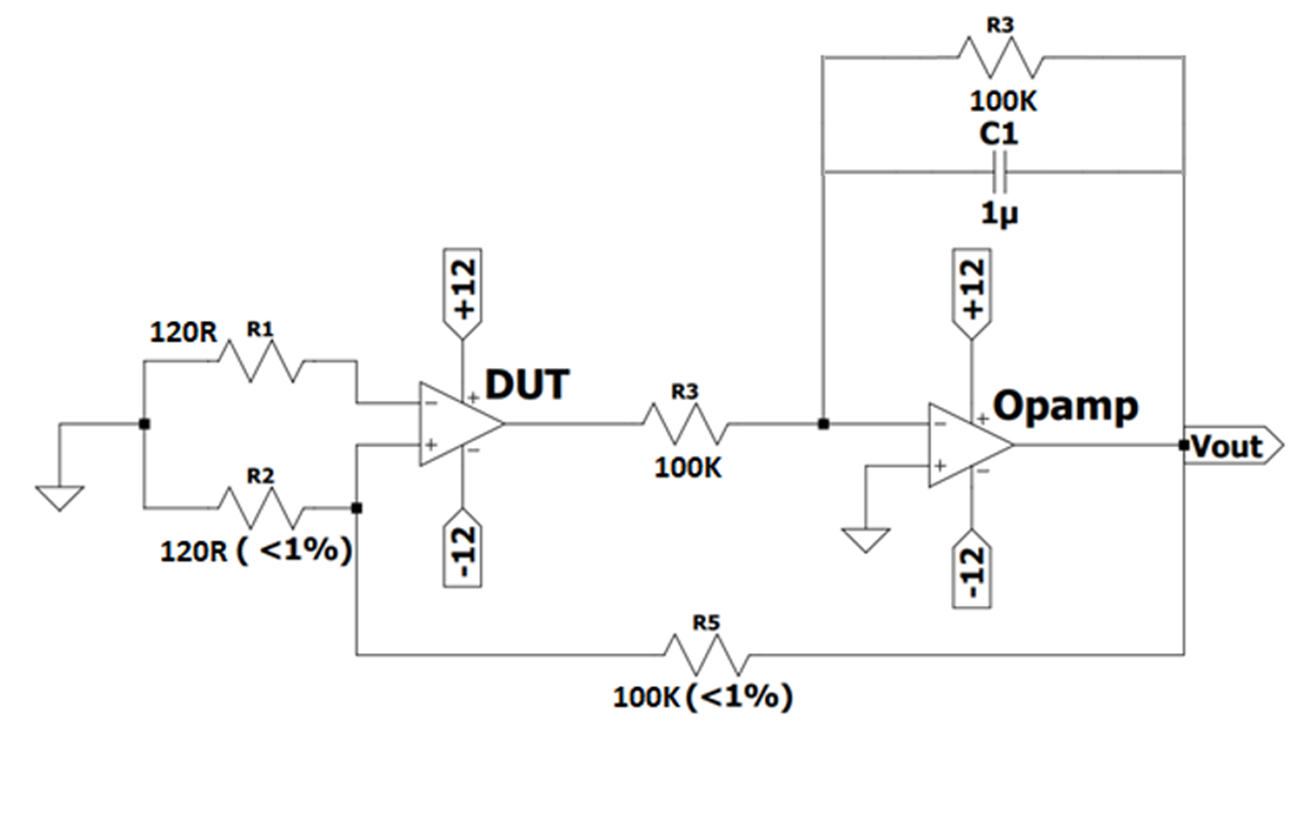
\includegraphics[width=0.7\textwidth]{IMAGEs/vos_test_circuit.png}
  \captionof{figure}{Figure 1: Input Offset Voltage Test Circuit for Op-Amp}
\end{center}

\begin{center}
  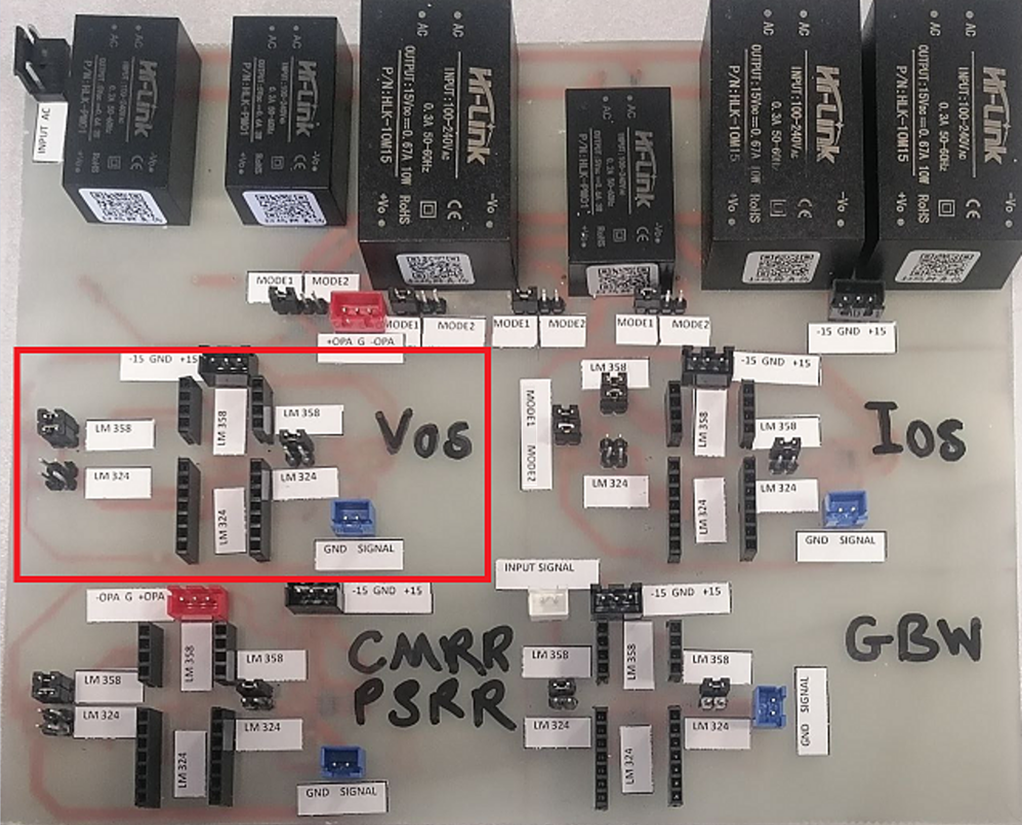
\includegraphics[width=0.6\textwidth]{IMAGEs/vos_test_device.png}
  \captionof{figure}{Figure 1: Input Offset Voltage Test Device for Op-Amp}
\end{center}

\subsection*{Formula for Calculating V\textsubscript{OS}}

\begin{equation}
V_{OS} = \frac{V_{out(DC)}}{\left(\frac{R_5}{R_2} + 1\right)}
\end{equation}

\section*{Instructions for Using the Test Device to Evaluate Op-Amp Quality}

\begin{itemize}
  \item The op-amp being tested for its offset voltage is referred to as the \textbf{DUT (Device Under Test)}.
  
  \item The precision of resistors R5 and R2 must be \textbf{1\% or better}. (If a new board is built, the exact values should be measured using an RLC meter and entered into the software for calibration.)

  \item The second op-amp used in the circuit, labeled \texttt{Opamp}, can be the same type as the DUT or a similar one. In this project, an \textbf{LM358} is used.

  \item Parameters and specifications should always be checked against the component's \textbf{datasheet}, since devices like the LM358 from different manufacturers (e.g., ST, Texas Instruments, Onsemi) may have slight variations.

  \item As shown in the figure, the test steps are clearly marked with \textbf{labels}. For instance, when testing LM324, jumpers should be set to the LM324 position; for LM358, the corresponding jumper setting should be selected.

  \item Power is supplied from the upper section of the board, clearly labeled. In this test, a supply of \textbf{$\pm$15V} is used exclusively.

  \item During the test, voltages must be \textbf{accurately measured} and entered into the software. The results are then exported to an Excel file.

  \item In the software interface, the relevant parameter (here, \texttt{Vof}) is first selected.

\begin{center}
  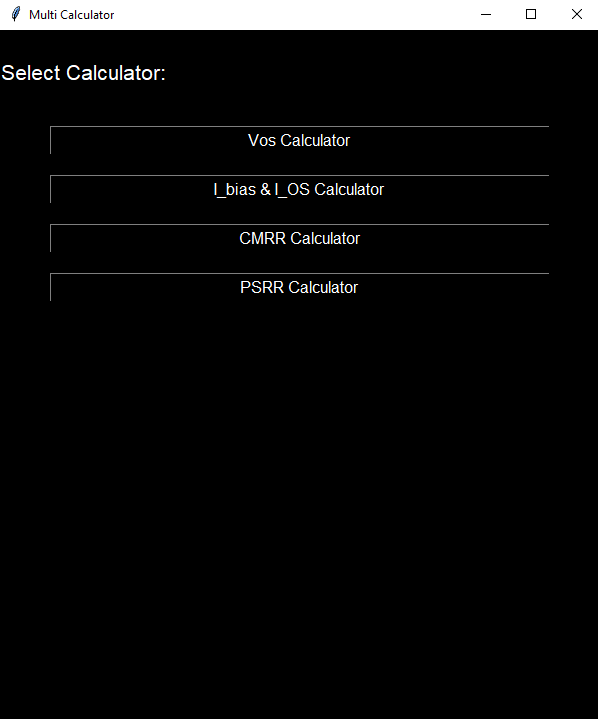
\includegraphics[width=0.4\textwidth]{IMAGEs/vos_software.png}
  \captionof{figure}{Figure 1: Input Offset Voltage Test Circuit for Op-Amp}
\end{center}

  \item In the next step, the measured values are entered and the results are recorded.

\begin{center}
  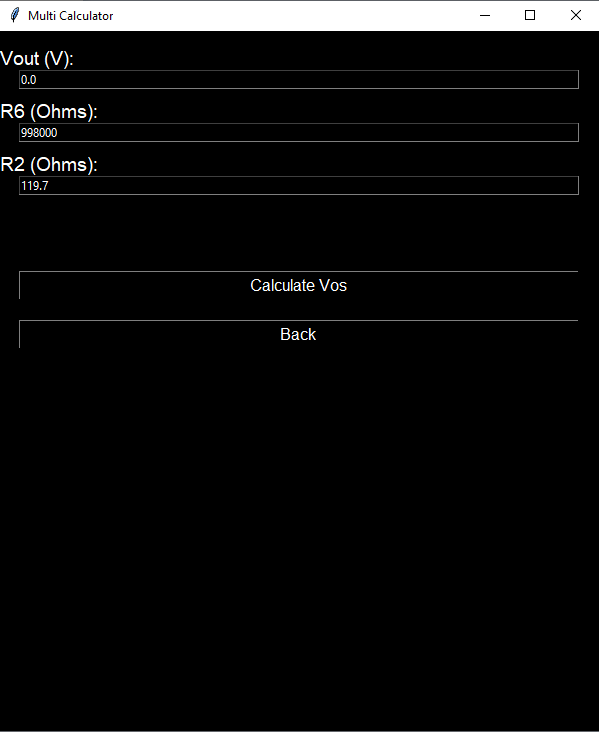
\includegraphics[width=0.4\textwidth]{IMAGEs/vos_software_setting.png}
  \captionof{figure}{Figure 1: Input Offset Voltage Test Circuit for Op-Amp}
\end{center}

\end{itemize}

\subsection*{Important Notes}

\begin{itemize}
  \item The values of resistors R2 and R5 are \textbf{fixed}. Under no circumstances should a new value be entered manually. If entered by mistake, restart the software to restore default values.

  \item You are only allowed to update resistor values if \textbf{a new resistor has been soldered to the board}. In such cases, the new values must be measured with an RLC meter and updated in the software.

  \item The software interface displays the \textbf{units of input and output values}. Ensure all values are entered and recorded using the correct units.
\end{itemize}

\newpage
\section{Input Offset Current Measurement (I\textsubscript{OS})}

To measure the input offset current of the operational amplifier, the following schematic is used:

\begin{center}
  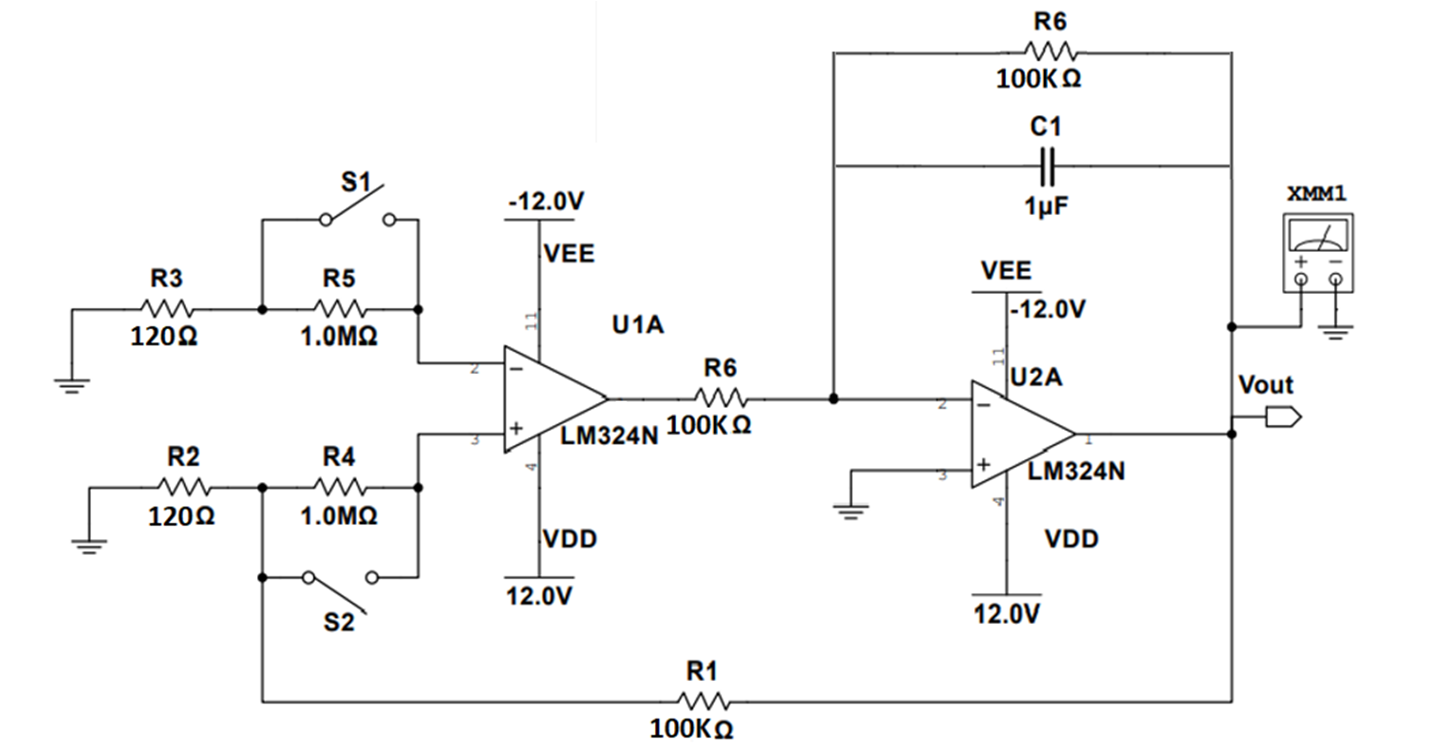
\includegraphics[width=0.7\textwidth]{IMAGEs/ios_test_circuit.png}
  \captionof{figure}{Figure 1: General Setup for Input Offset Current Measurement}
\end{center}

\begin{center}
  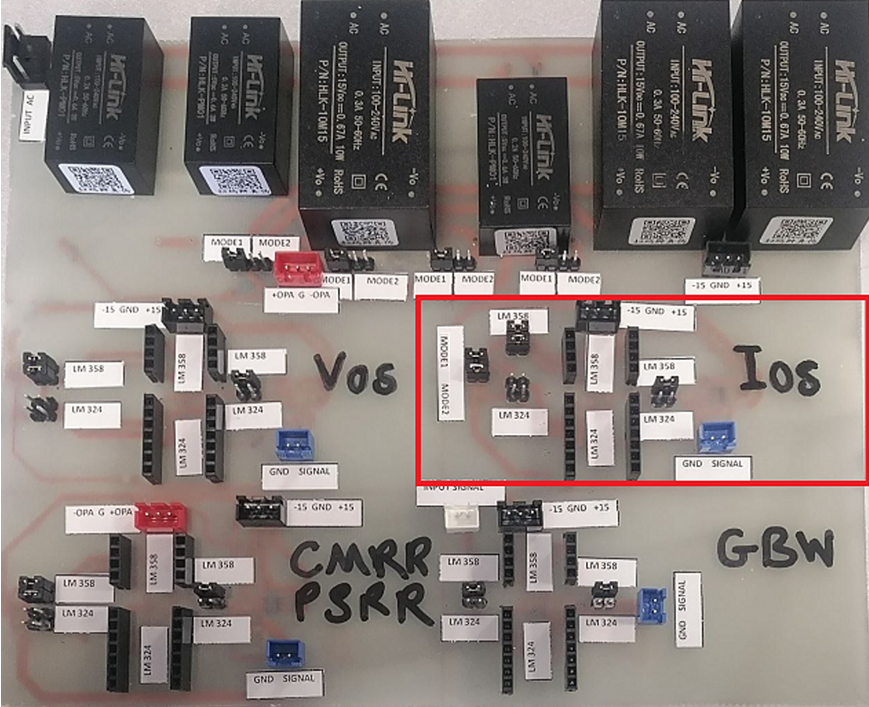
\includegraphics[width=0.5\textwidth]{IMAGEs/ios_test_device.png}
  \captionof{figure}{Figure 2: Offset Current Test Schematic}
\end{center}

\subsection*{Test Procedure and Recommendations}

\begin{itemize}
  \item Use precision resistors with minimal tolerance preferably \(\leq 1\%\) to ensure accurate current measurements.
  \item If any resistor or the test board is modified or replaced, the resistor values must be remeasured and updated in the software with high precision.
\end{itemize}

\subsection*{Step-by-Step Test Instructions for I\textsubscript{OS}}

The input offset current is measured in three stages by changing the switch configurations and recording output voltages:

\paragraph*{Stage 1: Both switches S1 and S2 are closed}
\begin{itemize}
  \item Short both ends of the resistors by closing S1 and S2.
  \item Both jumpers \texttt{mode1} and \texttt{mode2} are connected as per schematic.
  \item Record the output voltage as \( V_{outA} \).
\end{itemize}

\paragraph*{Stage 2: Open S1 and keep S2 closed}
\begin{itemize}
  \item Disconnect jumper \texttt{mode1} and leave \texttt{mode2} connected.
  \item Record the output voltage as \( V_{outB} \).
\end{itemize}

\paragraph*{Stage 3: Close S1 and open S2}
\begin{itemize}
  \item Disconnect jumper \texttt{mode2} and keep \texttt{mode1} connected.
  \item Record the output voltage as \( V_{outC} \).
\end{itemize}

\textbf{Note:} Always consider the polarity (positive or negative) of the voltages \( V_{outA}, V_{outB}, V_{outC} \) when entering values.

\subsection*{Hardware and Software Notes}

\begin{itemize}
  \item The secondary op-amp (labeled \texttt{Opamp}) can be the same as the DUT or a similar device. In this project, LM358 is used.
  \item Always verify datasheet specifications for the components used. For instance, LM358 variants from ST, Texas Instruments, and Onsemi may have slight differences.
  \item Test configuration labels (\texttt{Labels}) are clearly shown in the schematic:
    \begin{itemize}
      \item Set jumpers according to the device type (LM324 or LM358).
    \end{itemize}
  \item Power is supplied via the top labeled connector on the board. In this test, a supply of \( \pm15V \) is used.
  \item All voltage readings should be recorded precisely, entered into the software, and finally exported to an Excel sheet.
\end{itemize}

\begin{center}
  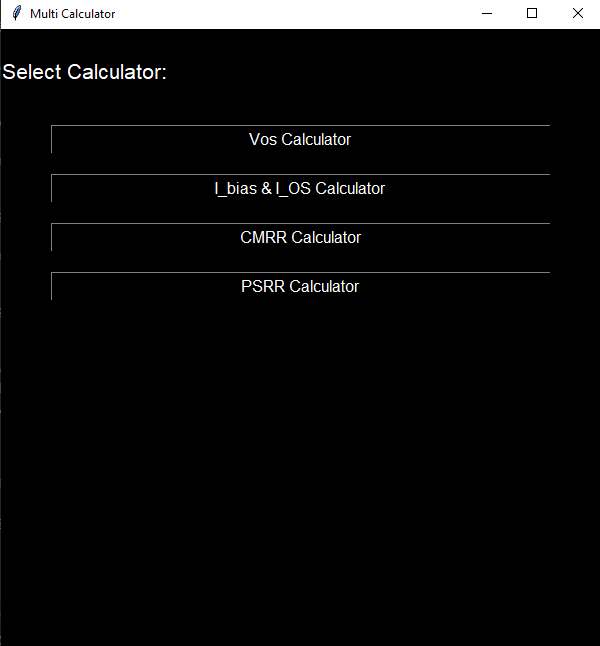
\includegraphics[width=0.5\textwidth]{IMAGEs/ios_software.png}
  \captionof{figure}{Figure 3: Software Interface – Select Ibias and Ios}
\end{center}

\begin{center}
  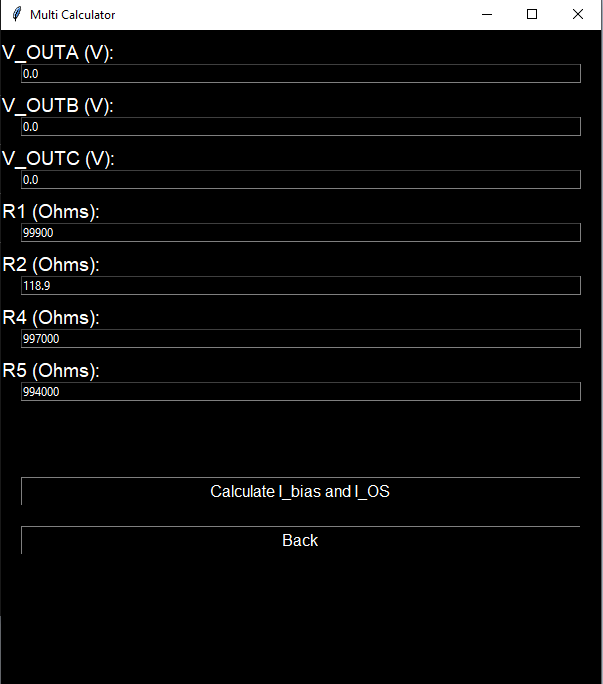
\includegraphics[width=0.5\textwidth]{IMAGEs/ios_software_entry.png}
  \captionof{figure}{Figure 4: Data Entry and Result Display}
\end{center}

\subsection*{Formulas for Bias and Offset Current Calculation}

The base bias currents for the inverting and non-inverting inputs are calculated using the following formulas:

\begin{align}
i_{b-} &= \frac{V_{outA} - V_{outB}}{R_5 \left( \frac{R_1 + R_2}{R_2} \right)} \\
i_{b+} &= \frac{V_{outC} - V_{outA}}{R_4 \left( \frac{R_1 + R_2}{R_2} \right)}
\end{align}

Or simplified:

\begin{align}
i_{b-} &= (V_{outA} - V_{outB}) \times 1.203 \times 10^{-9} \\
i_{b+} &= (V_{outC} - V_{outA}) \times 1.207 \times 10^{-9}
\end{align}

Then:

\begin{align}
I_{OS} &= i_{b+} - i_{b-} \\
I_{bias} &= \frac{i_{b+} + i_{b-}}{2}
\end{align}

\subsection*{Important Notes}

\begin{itemize}
  \item Resistors \( R_1, R_2, R_4, R_5 \) are fixed and must not be modified manually. If incorrect values are entered, restart the software to restore default settings.
  \item Only modify resistor values if new components are mounted on the board. In that case, measure accurately using an RLC meter and update values in the software.
  \item The software displays the units of all input and output fields. Always confirm that data is recorded using the correct units.
\end{itemize}

\newpage
\section{Common Mode Rejection Ratio (CMRR) Measurement}

To measure the Common Mode Rejection Ratio (CMRR) of an operational amplifier, the following circuit is used:

\begin{center}
  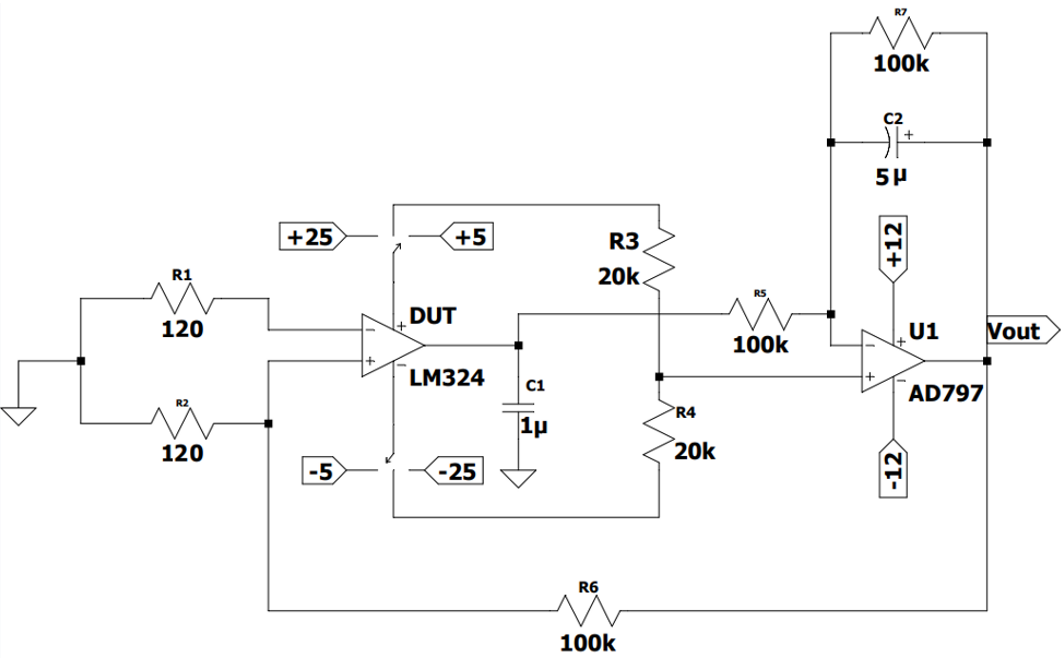
\includegraphics[width=0.7\textwidth]{IMAGEs/cmrr_test_circuit.png}
  \captionof{figure}{Figure: CMRR Test Circuit}
\end{center}

\subsection*{Formula for Calculating CMRR}

\begin{equation}
\text{CMRR} = 20 \cdot \log_{10} \left[ \left( \frac{R_6}{R_2} + 1 \right) \cdot \frac{20}{\Delta V_{out}} \right]
\end{equation}

\subsection*{Circuit and Measurement Considerations}

\begin{itemize}
  \item The secondary op-amp (labeled \texttt{Opamp} in the schematic) can be the same type as the DUT or a similar one. In this project, LM358 is used due to acceptable accuracy and availability.
  \item Ideally, the secondary op-amp should have high gain and low input offset voltage to ensure maximum measurement precision.
\end{itemize}

\subsection*{Op-Amp Datasheet Verification}

\begin{itemize}
  \item Always refer to the official datasheet for component parameters and tolerances.
  \item Identical models may have slight differences depending on the manufacturer. For example, LM358 is produced by STMicroelectronics, Texas Instruments, and Onsemi — each with minor electrical variations.
\end{itemize}

\subsection*{Test Configuration and Jumper Setup}

\begin{itemize}
  \item The test procedure is clearly marked using \texttt{Labels} in the schematic.
  \item When testing LM324, set the jumpers to the LM324 position.
  \item When testing LM358, use the appropriate LM358 jumper settings.
\end{itemize}

\subsection*{Power Supply Setup}

\begin{itemize}
  \item The required power is supplied through the labeled \texttt{Power} section on top of the board.
  \item In this test, a dual power supply of \( \pm15V \) is used.
\end{itemize}

\subsection*{Measurement Procedure for CMRR}

\begin{itemize}
  \item The op-amp is tested under two different supply conditions:
  \begin{itemize}
    \item First configuration: \( +25V, -5V \); record the output voltage as \( V_{out1} \)
    \item Second configuration: \( +5V, -25V \); record the output voltage as \( V_{out2} \)
  \end{itemize}
  \item Switching between configurations is done via jumper modes (Mode1 → Mode2), as clearly marked on the PCB.
  \item The absolute value of the output voltage difference \( |V_{out1} - V_{out2}| \) is used as \( \Delta V_{out} \) in the CMRR formula.
\end{itemize}

\subsection*{Software Operation for CMRR Test}

\begin{itemize}
  \item In the software, first select the parameter labeled \texttt{CMRR} from the test list.

  \begin{center}
    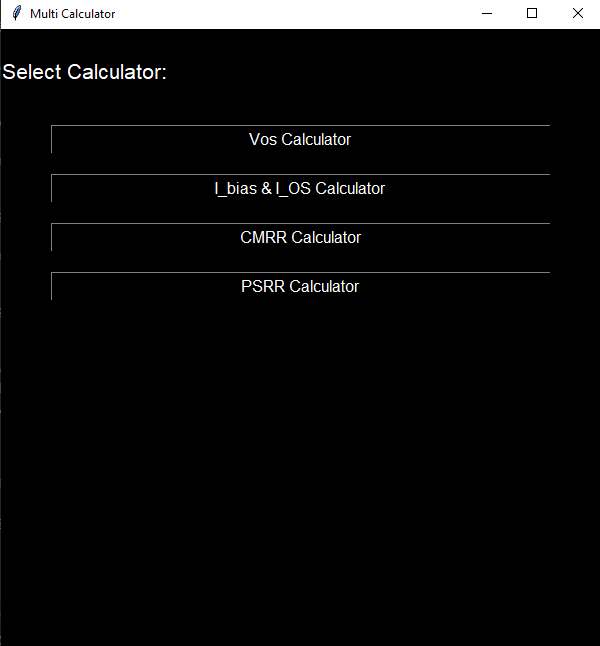
\includegraphics[width=0.6\textwidth]{IMAGEs/cmrr_software_select.png}
    \captionof{figure}{Figure: Selecting CMRR in Software}
  \end{center}

  \item Next, input the measured values of \( V_{out1} \) and \( V_{out2} \). The software automatically calculates \( \Delta V_{out} \) and computes the final CMRR value.

  \item For accurate measurement of small voltages, use the millivolt range of the multimeter.

  \begin{center}
    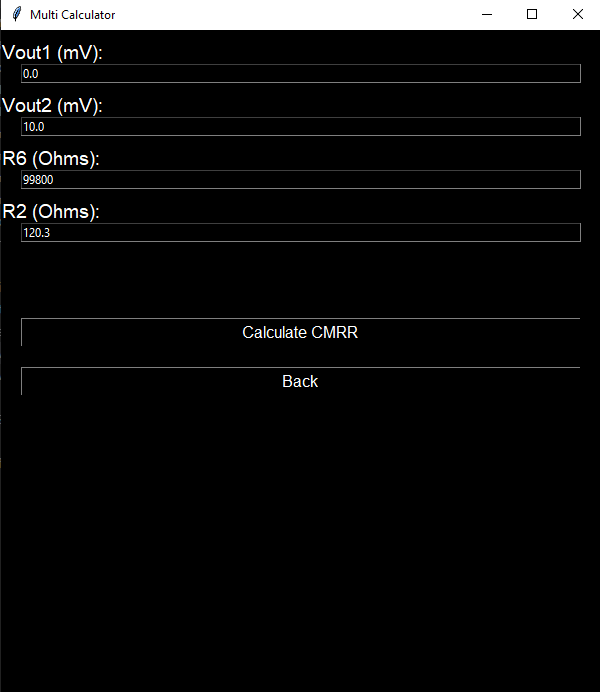
\includegraphics[width=0.6\textwidth]{IMAGEs/cmrr_software_entry.png}
    \captionof{figure}{Figure: Voltage Entry for CMRR Calculation}
  \end{center}
\end{itemize}

\subsection*{Important Notes}

\begin{itemize}
  \item The resistor values \( R_2 \) and \( R_6 \) are fixed and must not be manually changed in the software. If new values are entered by mistake, restart the application to restore defaults.
  \item Only update resistor values if new components have been soldered onto the board. In that case, accurately measure them using an RLC meter and update the software accordingly.
  \item The software clearly displays the units for all input and output fields. Always confirm that all values are entered and recorded using the correct units.
\end{itemize}

\newpage
\section{Power Supply Rejection Ratio (PSRR) Measurement}

The Power Supply Rejection Ratio (PSRR) is measured using a circuit similar to the one used for CMRR testing.  
Since the PSRR test range overlaps with the CMRR test conditions, verifying CMRR implicitly confirms the PSRR behavior — hence a separate PSRR calculation is often not necessary.

\begin{tcolorbox}[colback=yellow!5!white, colframe=yellow!80!black, title=Note]
The following steps are not required for routine testing. They are presented here only for completeness and demonstration purposes.
\end{tcolorbox}

\subsection*{Power Supply Configuration for PSRR Testing}

The test is carried out in two steps by varying the dual power supply:

\begin{itemize}
  \item \textbf{Step 1:} Set the power supply to \( \pm14V \) and measure the output voltage. Record the result as \( V_{out1} \).
  \item \textbf{Step 2:} Set the power supply to \( \pm15V \) and measure the new output voltage. Record the result as \( V_{out2} \).
  \item Calculate the absolute voltage difference: \( \Delta V_{out} = |V_{out1} - V_{out2}| \)
\end{itemize}

\subsection*{Data Entry in the Software}

\begin{itemize}
  \item From the software interface, select the \texttt{PSRR} option in the parameter menu.
  \item Input the measured values for \( V_{out1} \) and \( V_{out2} \). The software will automatically calculate \( \Delta V_{out} \) and compute the PSRR.
  \item The final result is stored in the PSRR section and exported to an Excel report.
\end{itemize}

\textbf{Tip:} For improved accuracy in measuring small voltage differences, use the millivolt range of the multimeter.

\subsection*{Formula for Calculating PSRR}

\begin{equation}
\text{PSRR} = 20 \cdot \log_{10} \left[ \left( \frac{R_6}{R_2} + 1 \right) \cdot \frac{1}{\Delta V_{out}} \right]
\end{equation}

\clearpage
\section{Gain Bandwidth Product (GBP) Measurement}

To measure the Gain Bandwidth Product (GBP) of the operational amplifier, a signal generator is required.

\begin{center}
  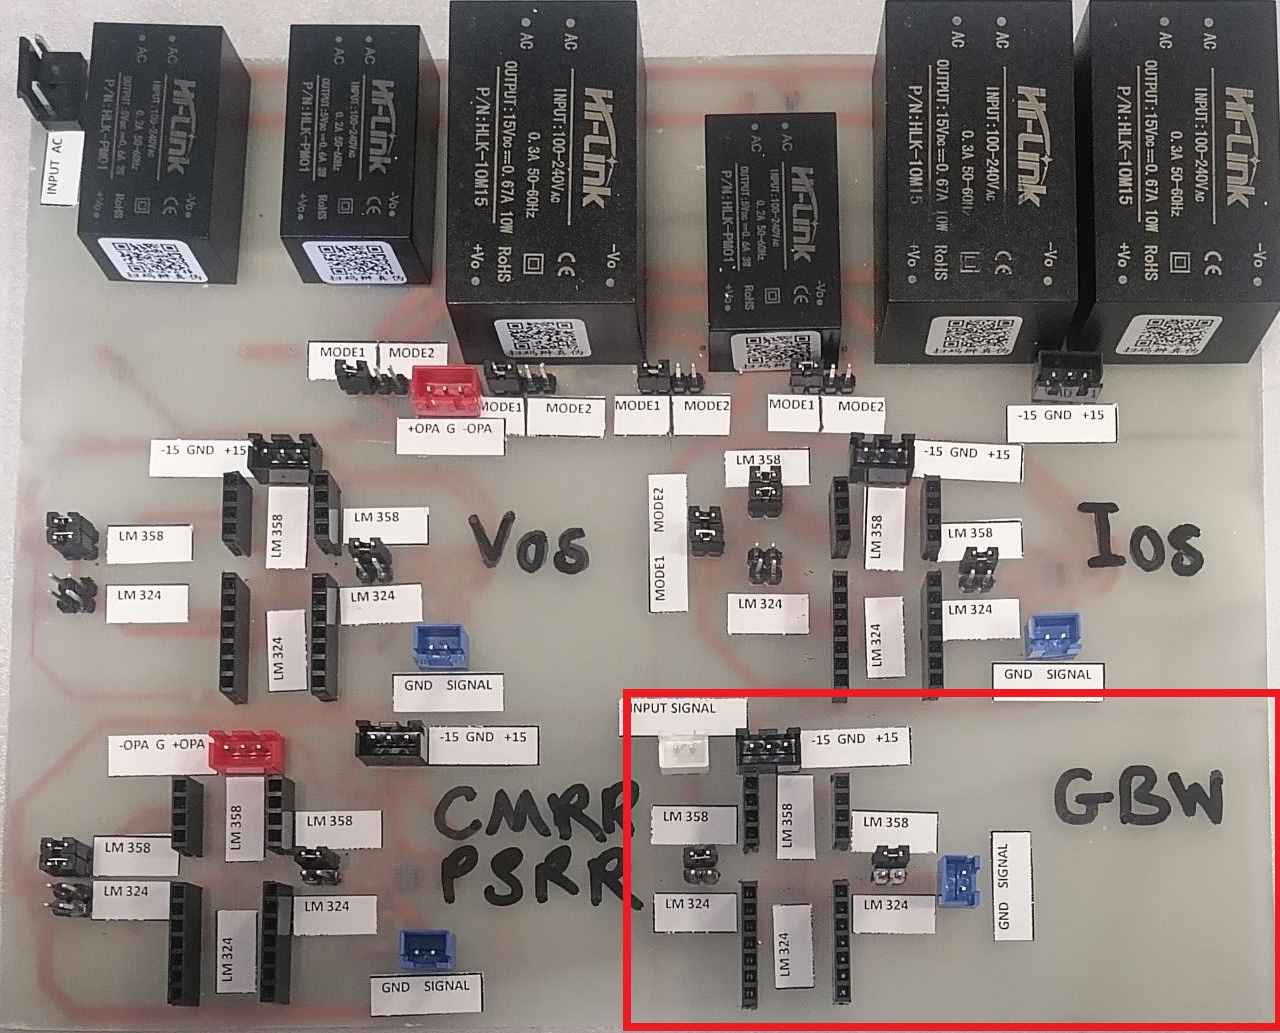
\includegraphics[width=0.7\textwidth]{IMAGEs/gbp_test_circuit.png}
  \captionof{figure}{Figure: GBP Test Circuit}
\end{center}

\begin{center}
  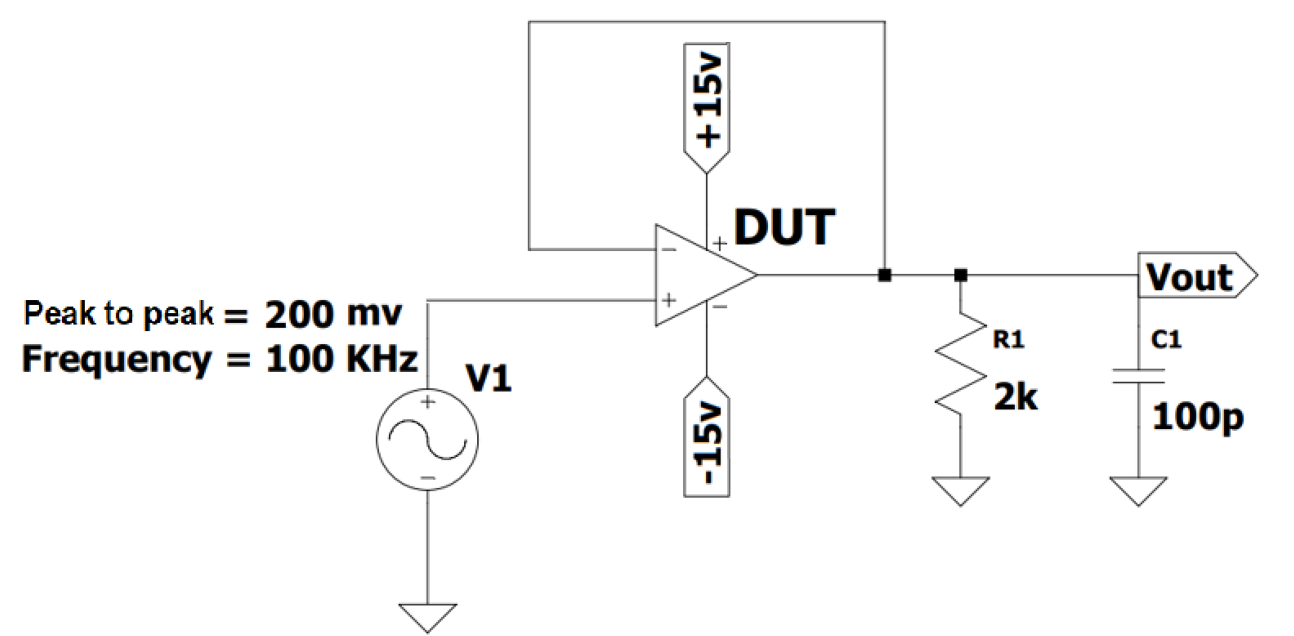
\includegraphics[width=0.7\textwidth]{IMAGEs/gbp_test_device.png}
  \captionof{figure}{Figure: GBP Test Device}
\end{center}

\subsection*{Test Procedure}

\begin{itemize}
  \item Connect the op-amp as shown in the circuit above.
  \item Gradually increase the input signal frequency using a signal generator.
  \item Monitor the output waveform on an oscilloscope.
  \item When the output signal’s peak-to-peak amplitude reaches approximately 140 millivolts, record the input frequency.
  \item This frequency corresponds to the Gain Bandwidth Product (GBP) of the op-amp under test.
\end{itemize}

\begin{tcolorbox}[colback=yellow!5!white, colframe=yellow!80!black, title=Note]
This test device is specifically designed for the listed parameters. For other op-amp parameters not included in this document, please refer to the previous test protocols and datasheets.
\end{tcolorbox}

\end{document}
